\clearpage\thispagestyle{empty}\SourceLeaf{002}
\vspace*{1cm}
\begin{center}\small
\textbf{CARL FRIEDRICH GAUSS WERKE}\\[1em]
\textbf{BAND III.}
\end{center}
\clearpage

\clearpage\thispagestyle{empty}\SourceLeaf{004}
\vspace*{1cm}
\begin{center}\small
\textbf{CARL FRIEDRICH GAUSS}\\[0.5em]
\textbf{WERKE}\\[1em]
\textbf{DRITTER BAND}\\[2em]
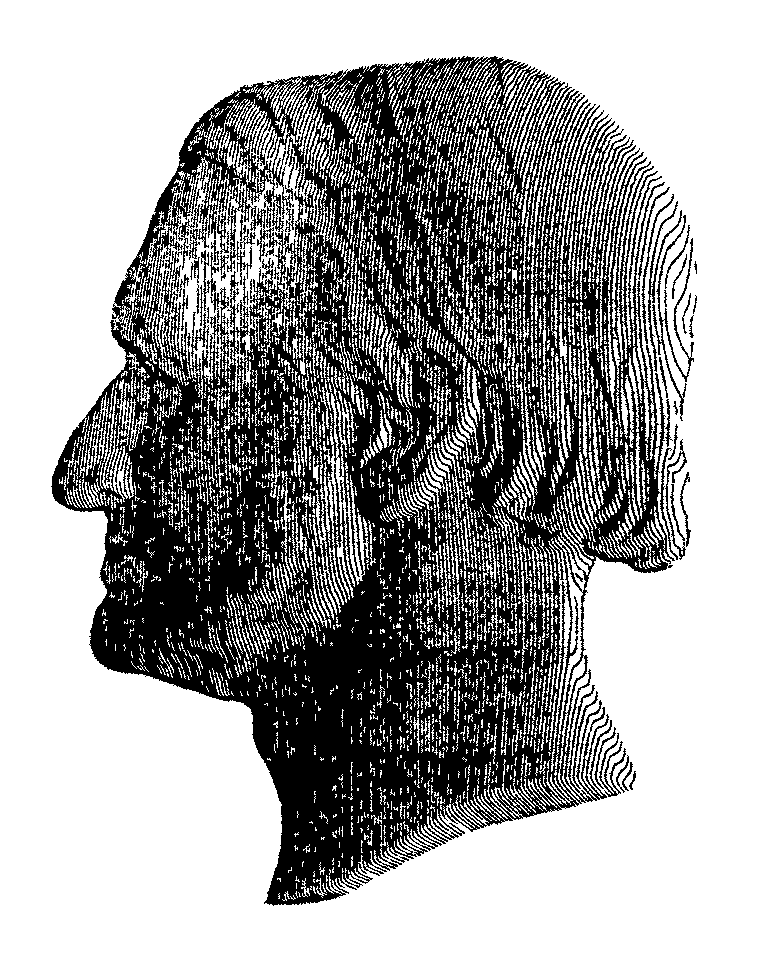
\includegraphics[width=1.65in]{assets/portrait_native004_complete.png}\\[2em]
\textbf{HERAUSGEGEBEN}\\[0.5em]
\textbf{VON DER}\\[0.5em]
\textbf{K\"ONIGLICHEN GESELLSCHAFT DER WISSENSCHAFTEN}\\[0.5em]
\textbf{ZU G\"OTTINGEN}\\[1em]
\textbf{1866.}
\end{center}
\clearpage

\clearpage\thispagestyle{empty}\SourceLeaf{006}
\vspace*{1cm}
\begin{center}\small
\textbf{DEMONSTRATIO NOVA}\\[0.75em]
\textbf{THEOREMATIS}\\[0.75em]
\textbf{OMNEM FUNCTIONEM ALGEBRAICAM}\\[0.5em]
\textbf{RATIONALEM INTEGRAM}\\[0.75em]
\textbf{UNIUS VARIABILIS}\\[0.75em]
\textbf{IN FACTORES REALES PRIMI VEL SECUNDI GRADUS}\\[0.75em]
\textbf{RESOLVI POSSE}\\[1.5em]
\textbf{QUAM PRO}\\[0.5em]
\textbf{OBTINENDIS SUMMIS IN PHILOSOPHIA HONORIBUS}\\[0.5em]
\textbf{INCLITO PHILOSOPHORUM ORDINI}\\[0.75em]
\textbf{ACADEMIAE IULIAE CAROLINAE}\\[1.5em]
\textbf{EXHIBUIT}\\[0.75em]
\textbf{CAROLUS FRIDERICUS GAUSS}\\[1.5em]
\rule{0.65\linewidth}{0.4pt}\\[0.75em]
\textbf{HELMSTADII}\\[0.5em]
\textbf{APUD C. G. FLECKEISEN. MDCCLXXXXIX.}
\end{center}

\clearpage
